\subsection{Diameter} \label{diameter}
In graph theory, \textit{shortest path} (SP) between node $a$ and $b$ of a graph is the minimum number of edges connecting them (i.e. the minimum number of ``steps'' to go from $a$ to $b$).
After computing SP for every couple of nodes in a graph, we can define \textit{diameter} as the maximum of the shortest paths.\\
As with clustering, we ran five  simulations for every memory size, obtaining a plot of diameter's mean over memory size with errors. Final regression will point out possible correlations.
\begin{figure}[h]
  \centering
  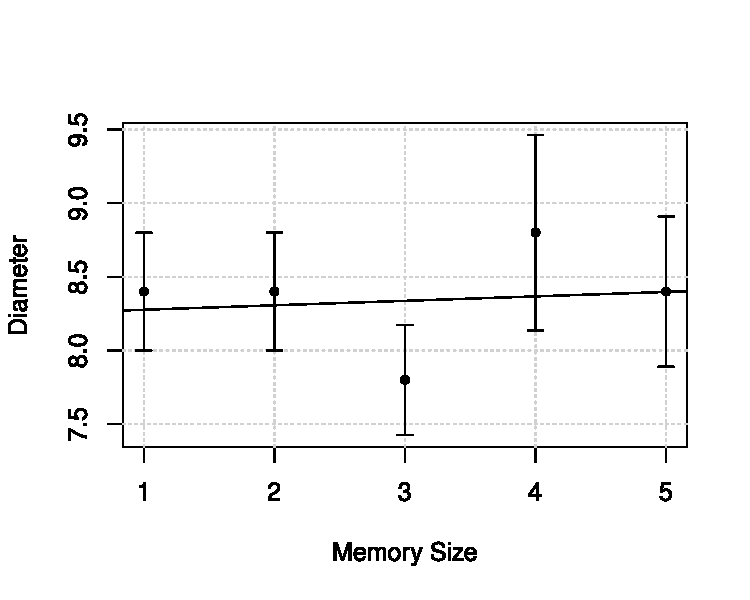
\includegraphics[trim={0cm 0cm 0cm 1cm},clip,width=.8\columnwidth]{img/diameter.pdf}
  \caption{diameter's mean-memory size linear weighted fit: five simulations per point}
  \label{fig:diameter}
\end{figure}


